\documentclass[dvipdfmx,aspectratio=169]{beamer}
\usepackage{pxjahyper}							%しおりの文字化けを防ぐ
\renewcommand{\kanjifamilydefault}{\gtdefault}	%日本語フォントをゴシックに
\usepackage{graphics}							%各種画像の張り込み
\usepackage{amsmath,amssymb,mathtools}					%標準数式表現を拡大する
\usepackage{ulem}
\usepackage{ascmac,fancybox}
\usetheme[
	block=fill,
	progressbar=foot,
	numbering=fraction,
	subsectionpage=progressbar
]{Metropolis}
\usefonttheme{professionalfonts}

\usepackage{here}
\usepackage{booktabs}

\usepackage{tikz}
\usetikzlibrary{positioning}
\usepackage{color}

\newcommand{\highlight}[2][yellow]{\tikz[baseline=(x.base)]{\node[rectangle,rounded corners,fill=#1!10](x){#2};}}
\newcommand{\highlightcap}[3][yellow]{\tikz[baseline=(x.base)]{\node[rectangle,rounded corners,fill=#1!10](x){#2} node[below of=x, color=#1]{#3};}}

\title{ディープラーニングの仕組みを知ろう!}
\subtitle{第3回 人工知能勉強会}
\author{Shion MORISHITA}
\institute{}
\date{\today}

\subject{\LaTeX{}+Beamer}
\begin{document}
	%タイトル
	\begin{frame}[plain]
	    \maketitle
	\end{frame}
		
	\begin{frame}[shrink]{目次}
		\vspace{1em}
		\tableofcontents
	\end{frame}
	
	\section{はじめに}
	\begin{frame}{目的}
		\begin{itemize}
			\item
		\end{itemize}
	\end{frame}
	
	\section{勾配降下法の復習}
	\begin{frame}{勾配降下法のイメージ}
		\underline{ボールが転がる方向に向かってパラメータ(ここでは$ x $)を更新}
		
		\begin{figure}
			\centering
			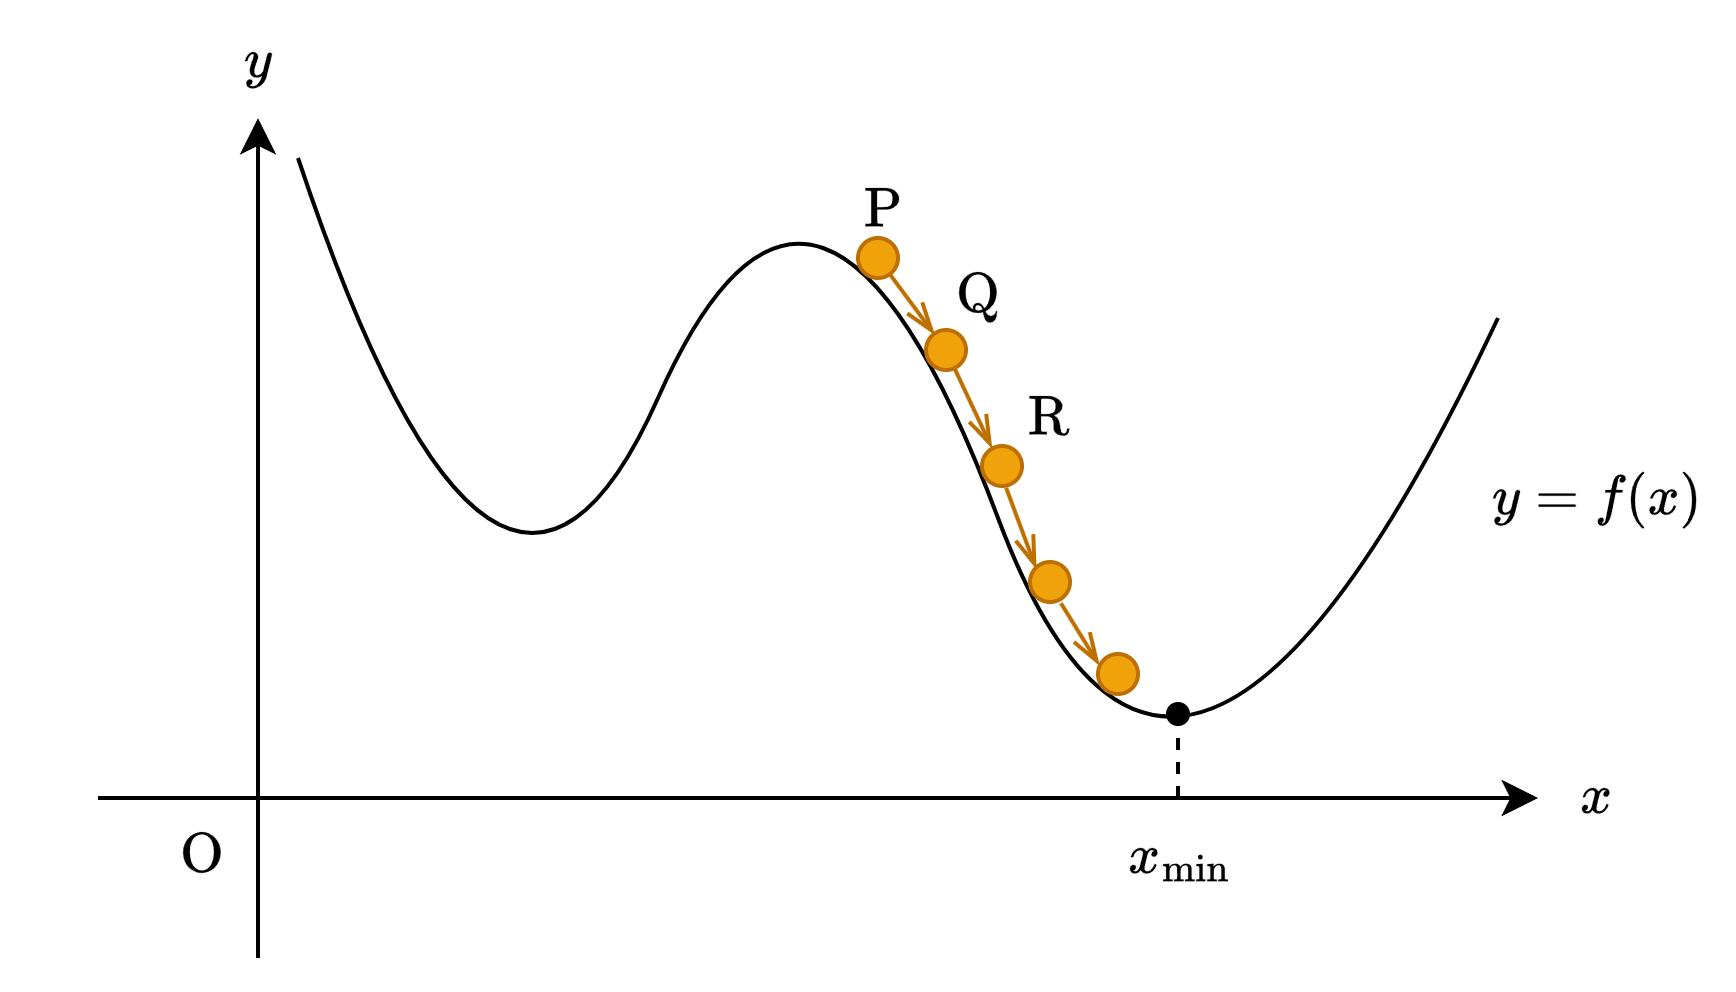
\includegraphics[width=0.7\linewidth]{img/image-of-a-ball-rolling-down-a-slope}
		\end{figure}
		
	\end{frame}
	\begin{frame}{ニューラルネットワークのパラメータ}
		\underline{$ w^2_{11}, \dots, w^3_{11}, \dots, b^2_1, \dots, b^3_1, \dots $がパラメータ}
		\begin{figure}
			\centering
			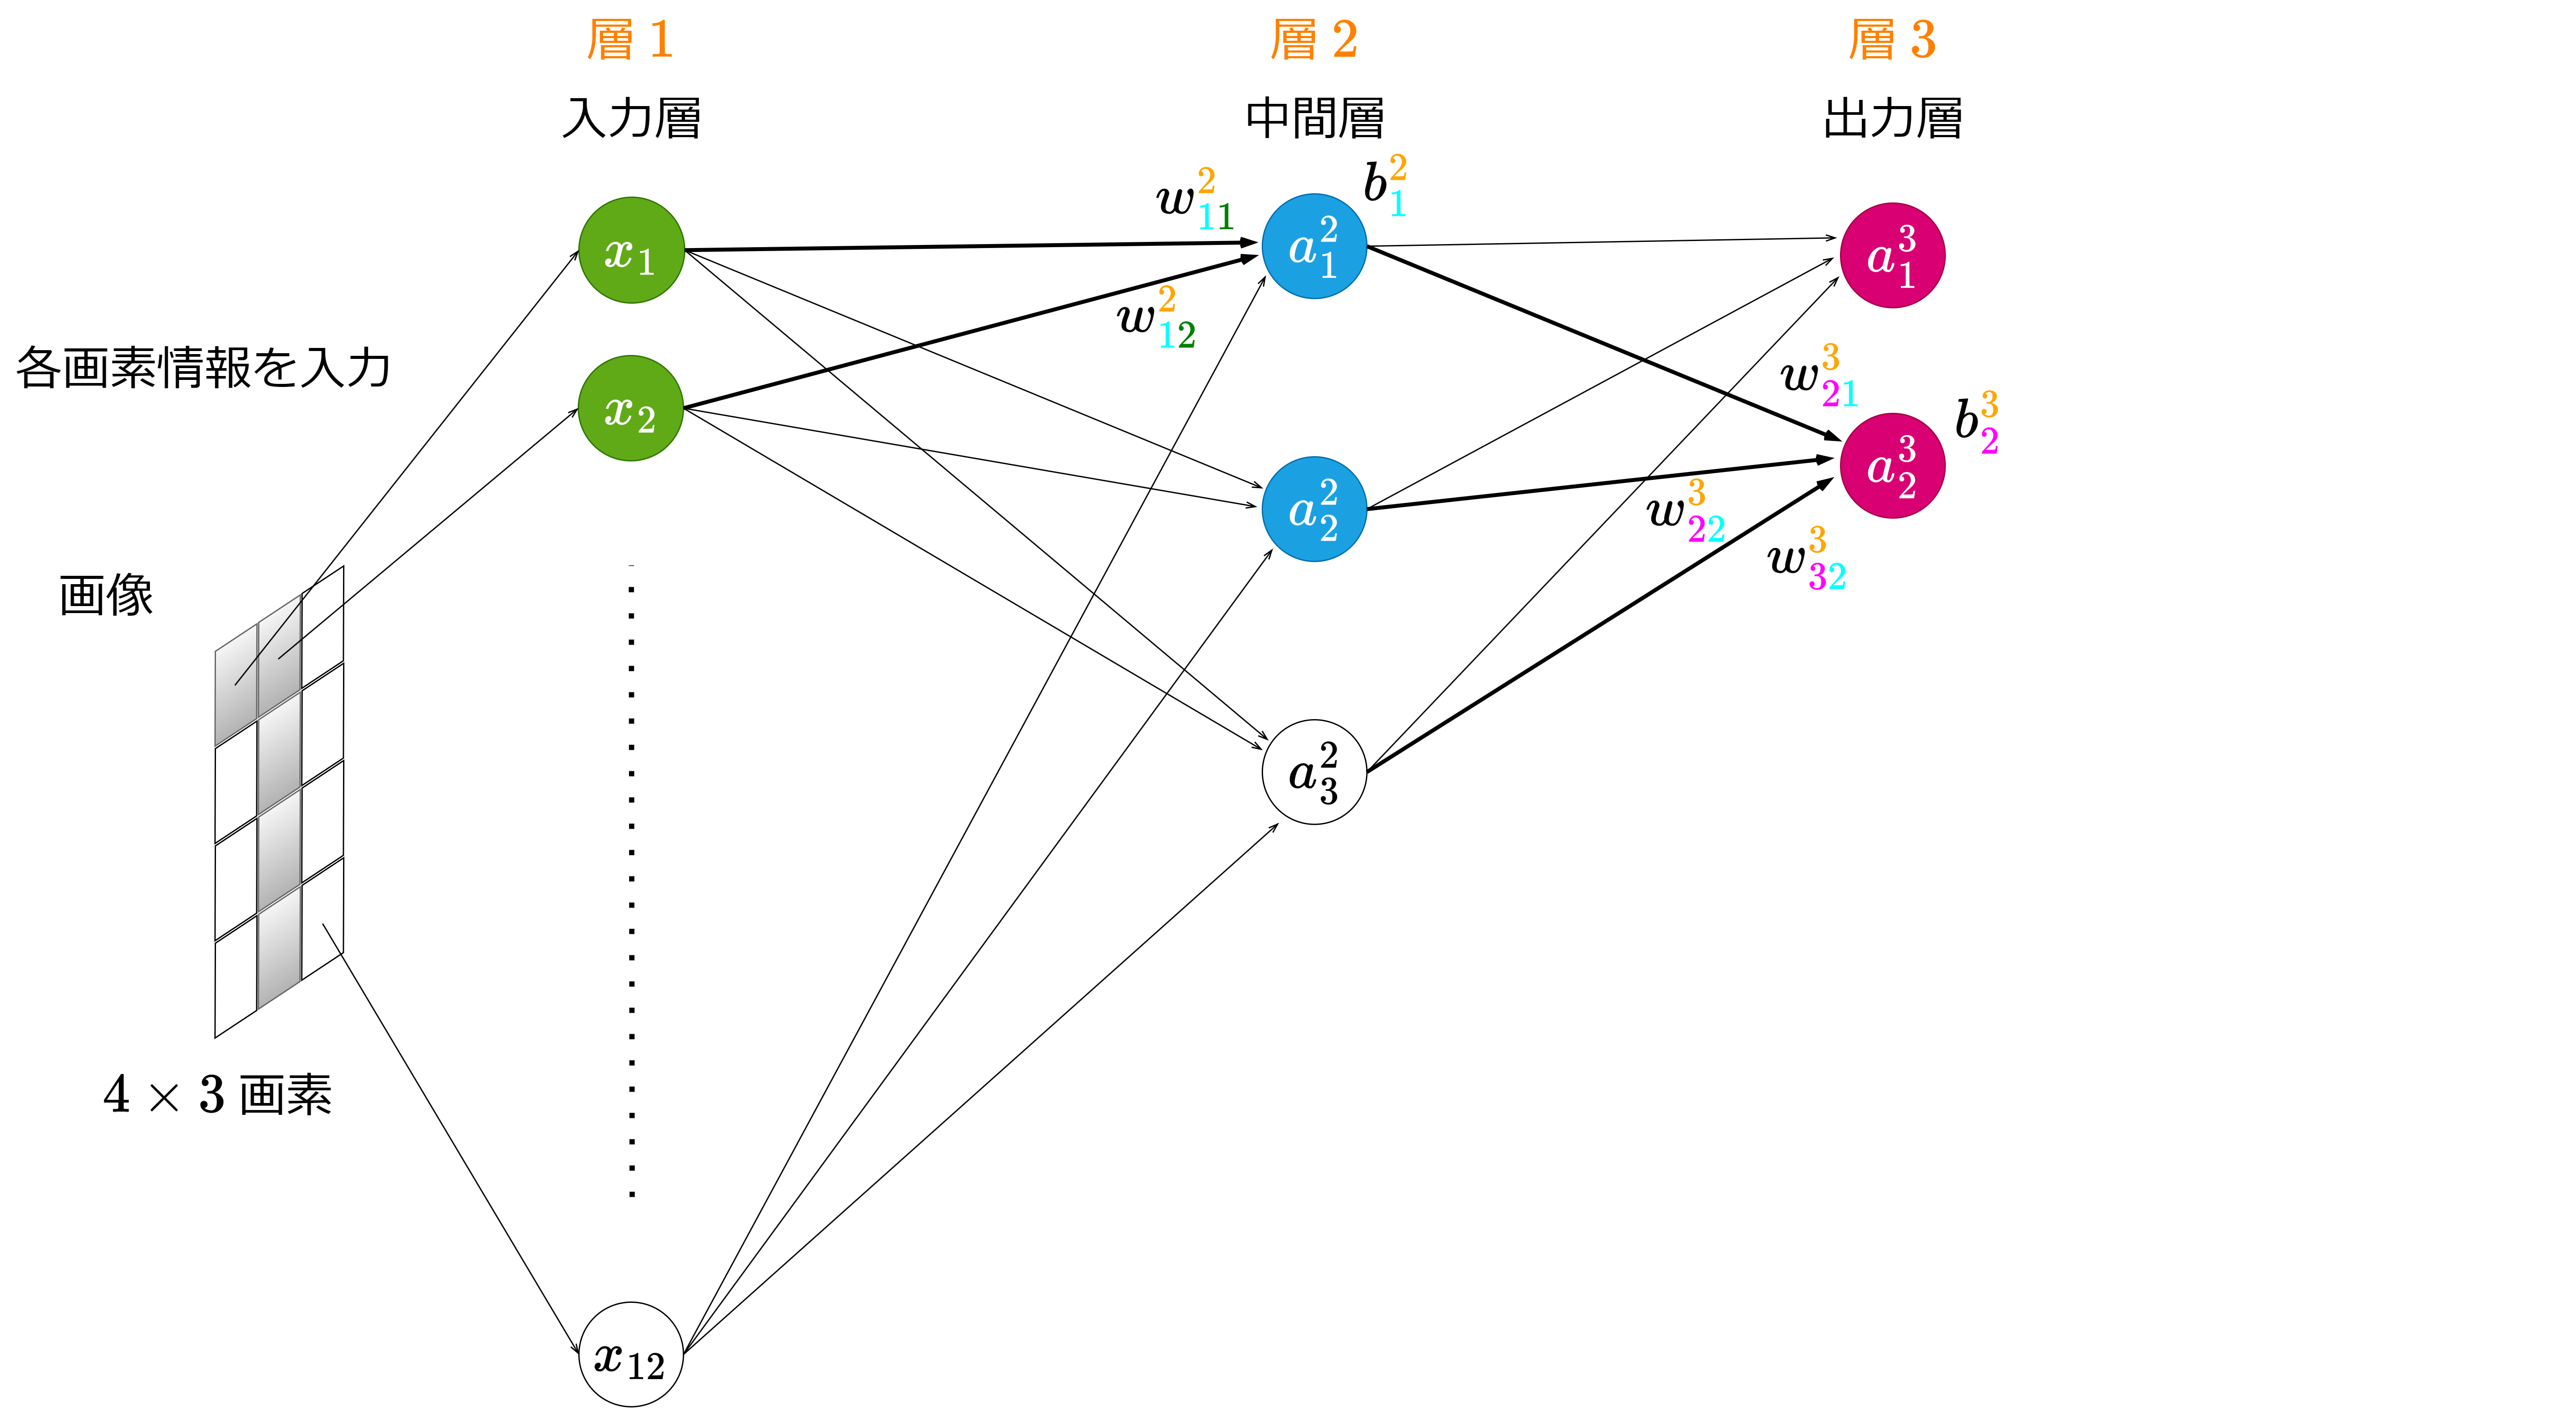
\includegraphics[width=0.8\linewidth]{img/illustration-of-variable-and-parameter-names}
		\end{figure}
	\end{frame}
	\begin{frame}{ニューラルネットワークへの勾配降下法の適用}
		$ \begin{bmatrix}
			\Delta w^2_{11}\\ \vdots\\
			\Delta w^3_{11}\\ \vdots\\
			\Delta b^2_1\\ \vdots\\
			\Delta b^3_1\\ \vdots
		\end{bmatrix} = -\eta \begin{bmatrix}
			\dfrac{\partial C_\mathrm{T}}{\partial w^2_{11}}\\ \vdots\\
			\dfrac{\partial C_\mathrm{T}}{\partial w^3_{11}}\\ \vdots\\
			\dfrac{\partial C_\mathrm{T}}{\partial b^2_1}\\ \vdots\\
			\dfrac{\partial C_\mathrm{T}}{\partial b^3_1}\\ \vdots\\
		\end{bmatrix} $を用いて、$ \begin{bmatrix}
			w^2_{11}\\ \vdots\\
			w^3_{11}\\ \vdots\\
			b^2_1\\ \vdots\\
			b^3_1\\ \vdots
		\end{bmatrix} $を$ \begin{bmatrix}
			w^2_{11} + \Delta w^2_{11}\\ \vdots\\
			w^3_{11} + \Delta w^3_{11}\\ \vdots\\
			b^2_1 + \Delta b^2_1\\ \vdots\\
			b^3_1 + \Delta b^3_1\\ \vdots
		\end{bmatrix} $へ更新を繰り返す。
		
		※正の小さな定数$ \eta $を\alert{学習係数}といい、モデル作成者が自由に設定する。
	\end{frame}
	\begin{frame}{勾配降下法の問題点}
		\underline{微分を実際に計算するのは大変}
		\begin{align*}
			\dfrac{\partial C_\mathrm{T}}{\partial w^2_{11}} 
			&= \sum_{k=1}^{64} \dfrac{\partial C_k}{\partial w^2_{11}}\\
			&= \sum_{k=1}^{64}\left\{ \dfrac{\partial C_k}{\partial a^3_1[k]}\dfrac{\partial a^3_1[k]}{\partial z^3_1[k]}\dfrac{\partial z^3_1[k]}{\partial a^2_1[k]}\dfrac{\partial a^2_1[k]}{\partial z^2_1[k]}\dfrac{\partial z^2_1[k]}{\partial w^2_{11}} + \dfrac{\partial C_k}{\partial a^3_2[k]}\dfrac{\partial a^3_2[k]}{\partial z^3_2[k]}\dfrac{\partial z^3_2[k]}{\partial a^2_1[k]}\dfrac{\partial a^2_1[k]}{\partial z^2_1[k]}\dfrac{\partial a^2_1[k]}{\partial w^2_{11}} \right\}.
		\end{align*}
	\end{frame}
	\begin{frame}{微分地獄の解決策}
		\underline{\alert{誤差逆伝播法} の導入}
		% TODO: \usepackage{graphicx} required
		\begin{figure}
			\centering
			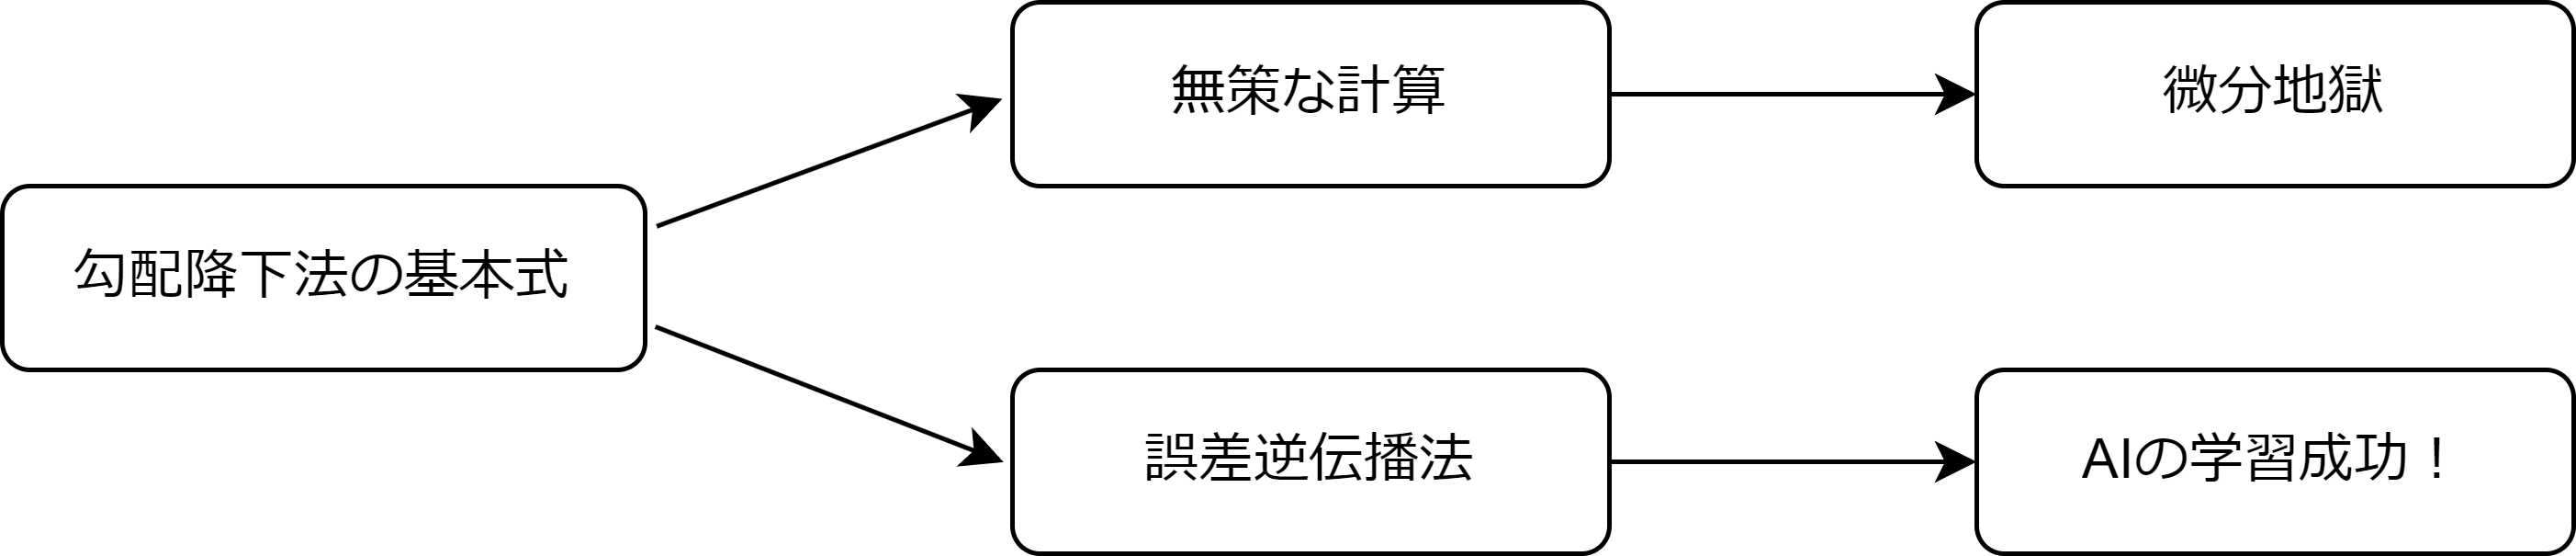
\includegraphics[width=0.9\linewidth]{img/positioning-of-the-error-back-propagation-method}
		\end{figure}
	\end{frame}
	
	\section{誤差逆伝播法}
	\subsection{ユニットの誤差}
	\begin{frame}{誤差逆伝播法とは?}
		\underline{特徴}
		\begin{itemize}
			\item 煩雑な微分計算を、\alert{数列の漸化式}に置き換える
			\item \alert{ユニットの誤差}(error)と呼ばれる変数$ \delta^l_j $を用いる
		\end{itemize}
	\end{frame}
	\begin{frame}{ユニットの誤差$ \delta^l_j $の導入}
		\begin{screen}
			\alert{ユニットの誤差}$ \delta^l_j $を次のように定義する:
			\begin{equation}\label{eq:unit-error}
				\delta^l_j \triangleq \dfrac{\partial C}{\partial z^l_j}
			\end{equation}
		\end{screen}
		なぜこれを導入したか?
		\begin{itemize}
			\item 微分の計算から漸化式の計算へ変えることができるから
		\end{itemize}		
	\end{frame}
	\begin{frame}{ユニットの誤差$ \delta^l_j $のイメージ}
		% TODO: \usepackage{graphicx} required
		\begin{figure}
			\centering
			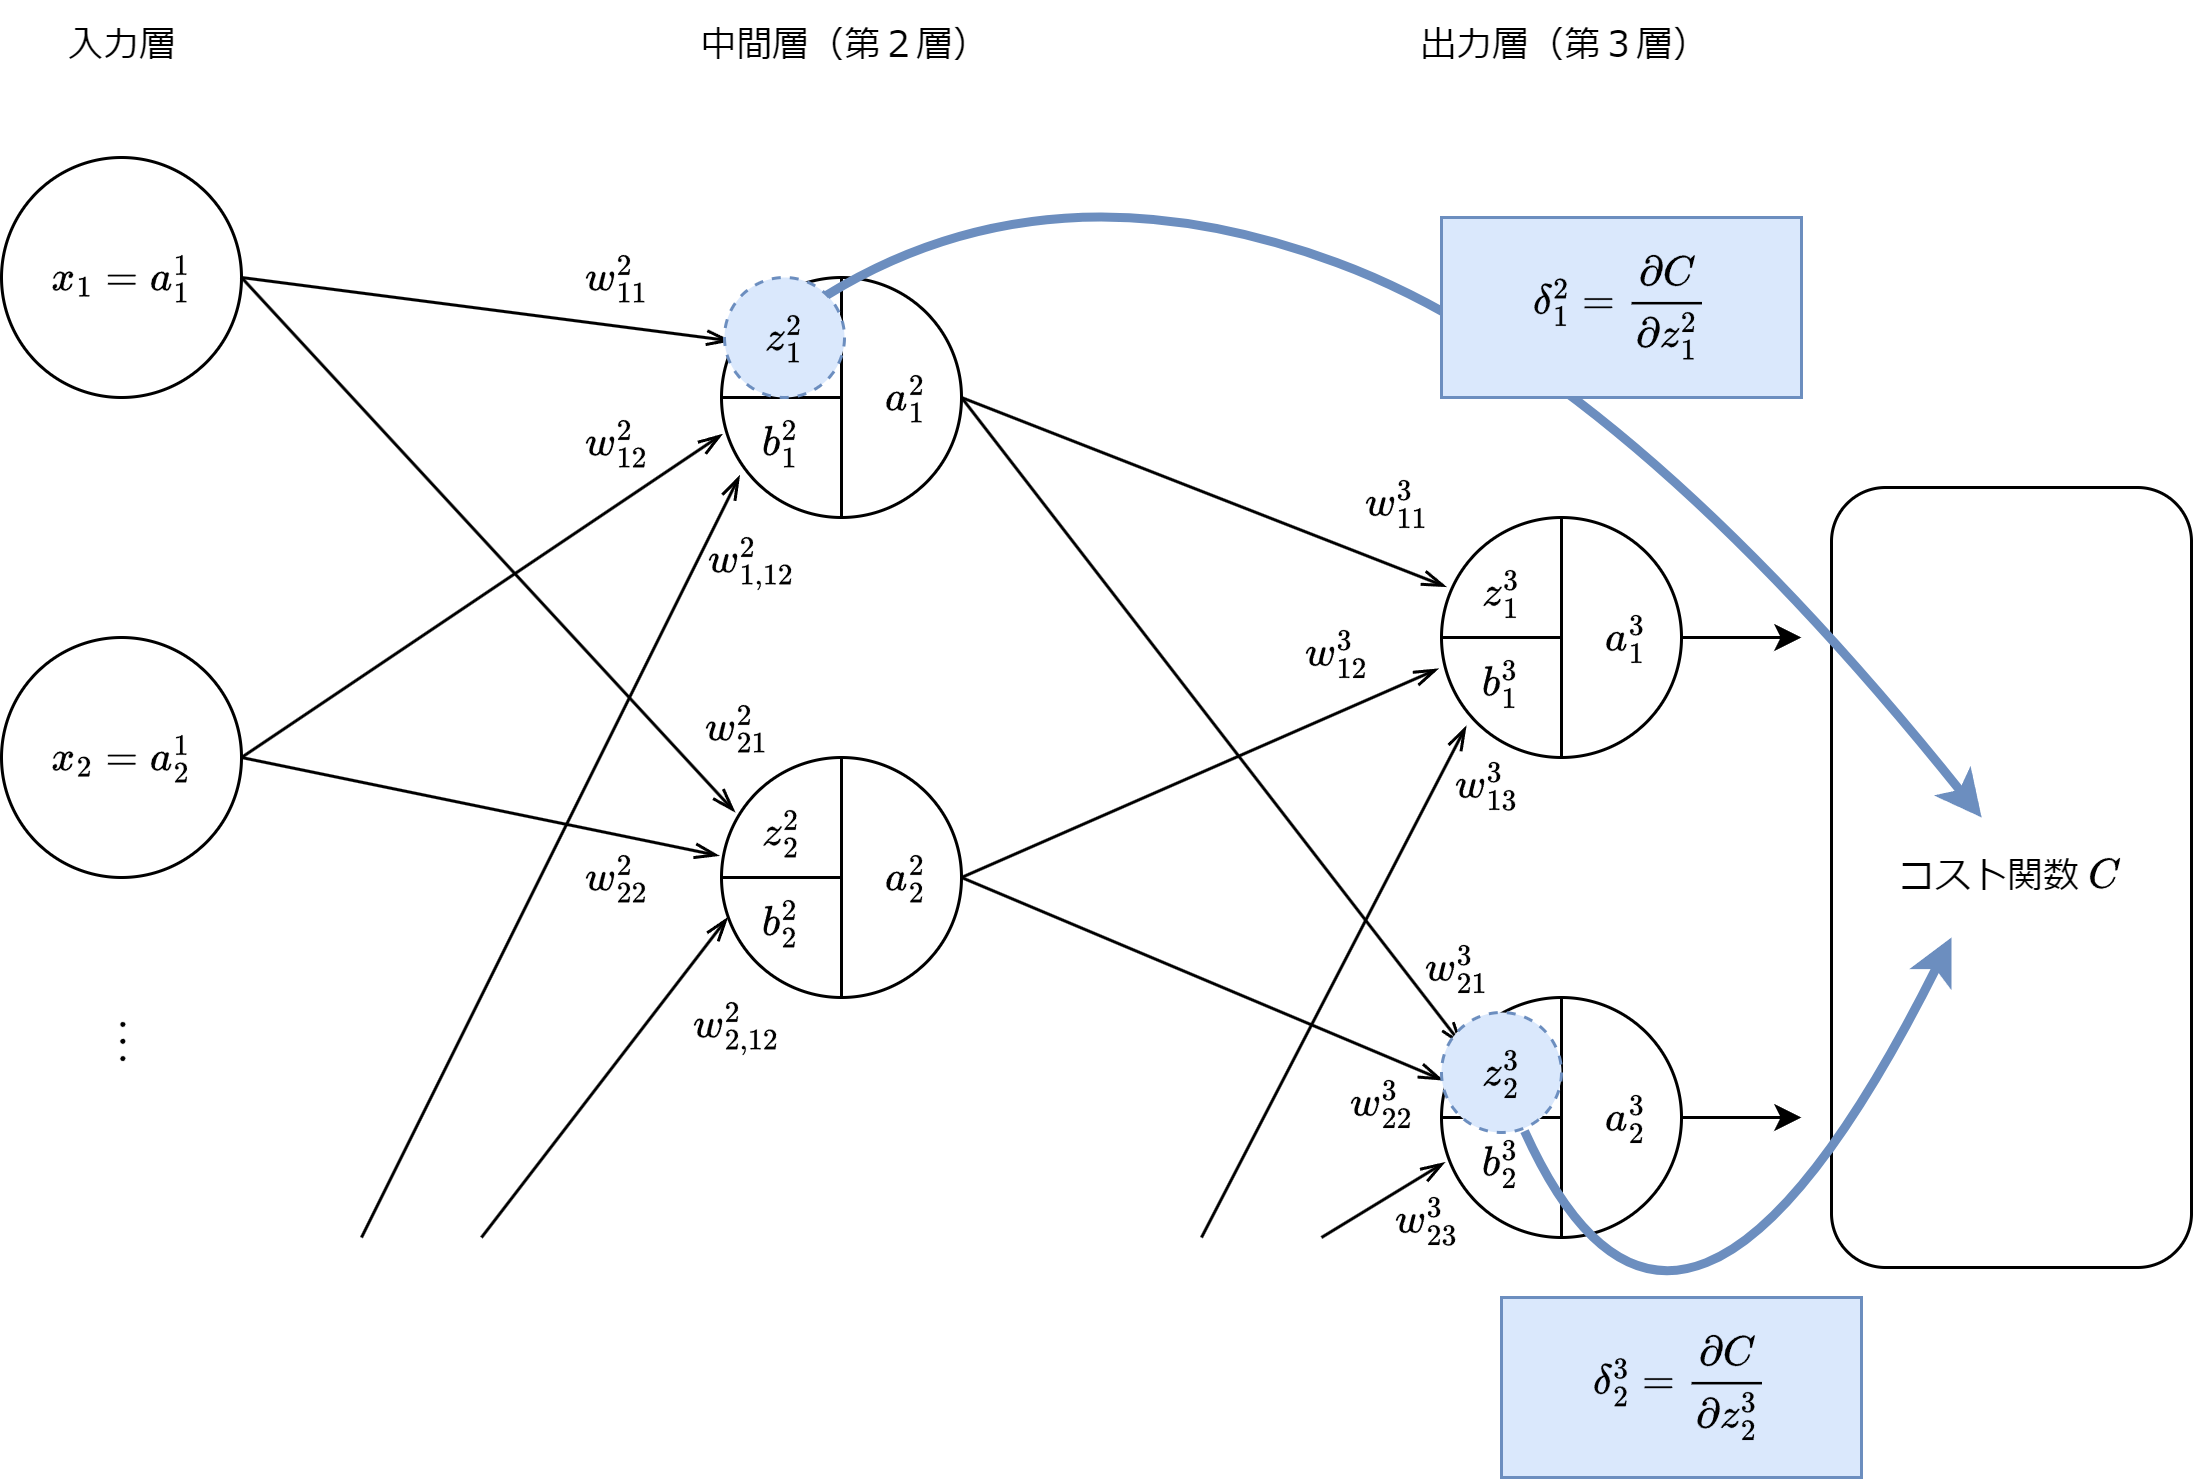
\includegraphics[width=0.7\linewidth]{img/image-of-unit-error}
		\end{figure}
	\end{frame}
	\begin{frame}{重みに関する2乗誤差の偏微分を$ \delta^l_j $で表現}
		\begin{screen}
			重みに関する偏微分をユニットの誤差$ \delta^l_j $を用いて次にように表すことができる:
			\begin{equation}\label{eq:equation-expressing-the-partial-derivative-with-respect-to-the-weights-using-the-unit-error}
				\dfrac{\partial C}{\partial w^l_{ji}} = \delta^l_j a^{l-1}_i\quad (l \geq 2).
			\end{equation}
		\end{screen}
		\underline{ポイント}
		\begin{itemize}
			\item $ \delta^l_j $の値さえ計算できれば、$ \dfrac{\partial C}{\partial w^l_{ji}} $を偏微分の計算なしで求めることができる!
			\begin{itemize}
				\item $ a^{l-1}_i $はユニットの出力値なので、普通に計算できる
			\end{itemize}
		\end{itemize}
	\end{frame}
	\begin{frame}{重みに関する2乗誤差の偏微分のイメージ}
		% TODO: \usepackage{graphicx} required
		\begin{figure}
			\centering
			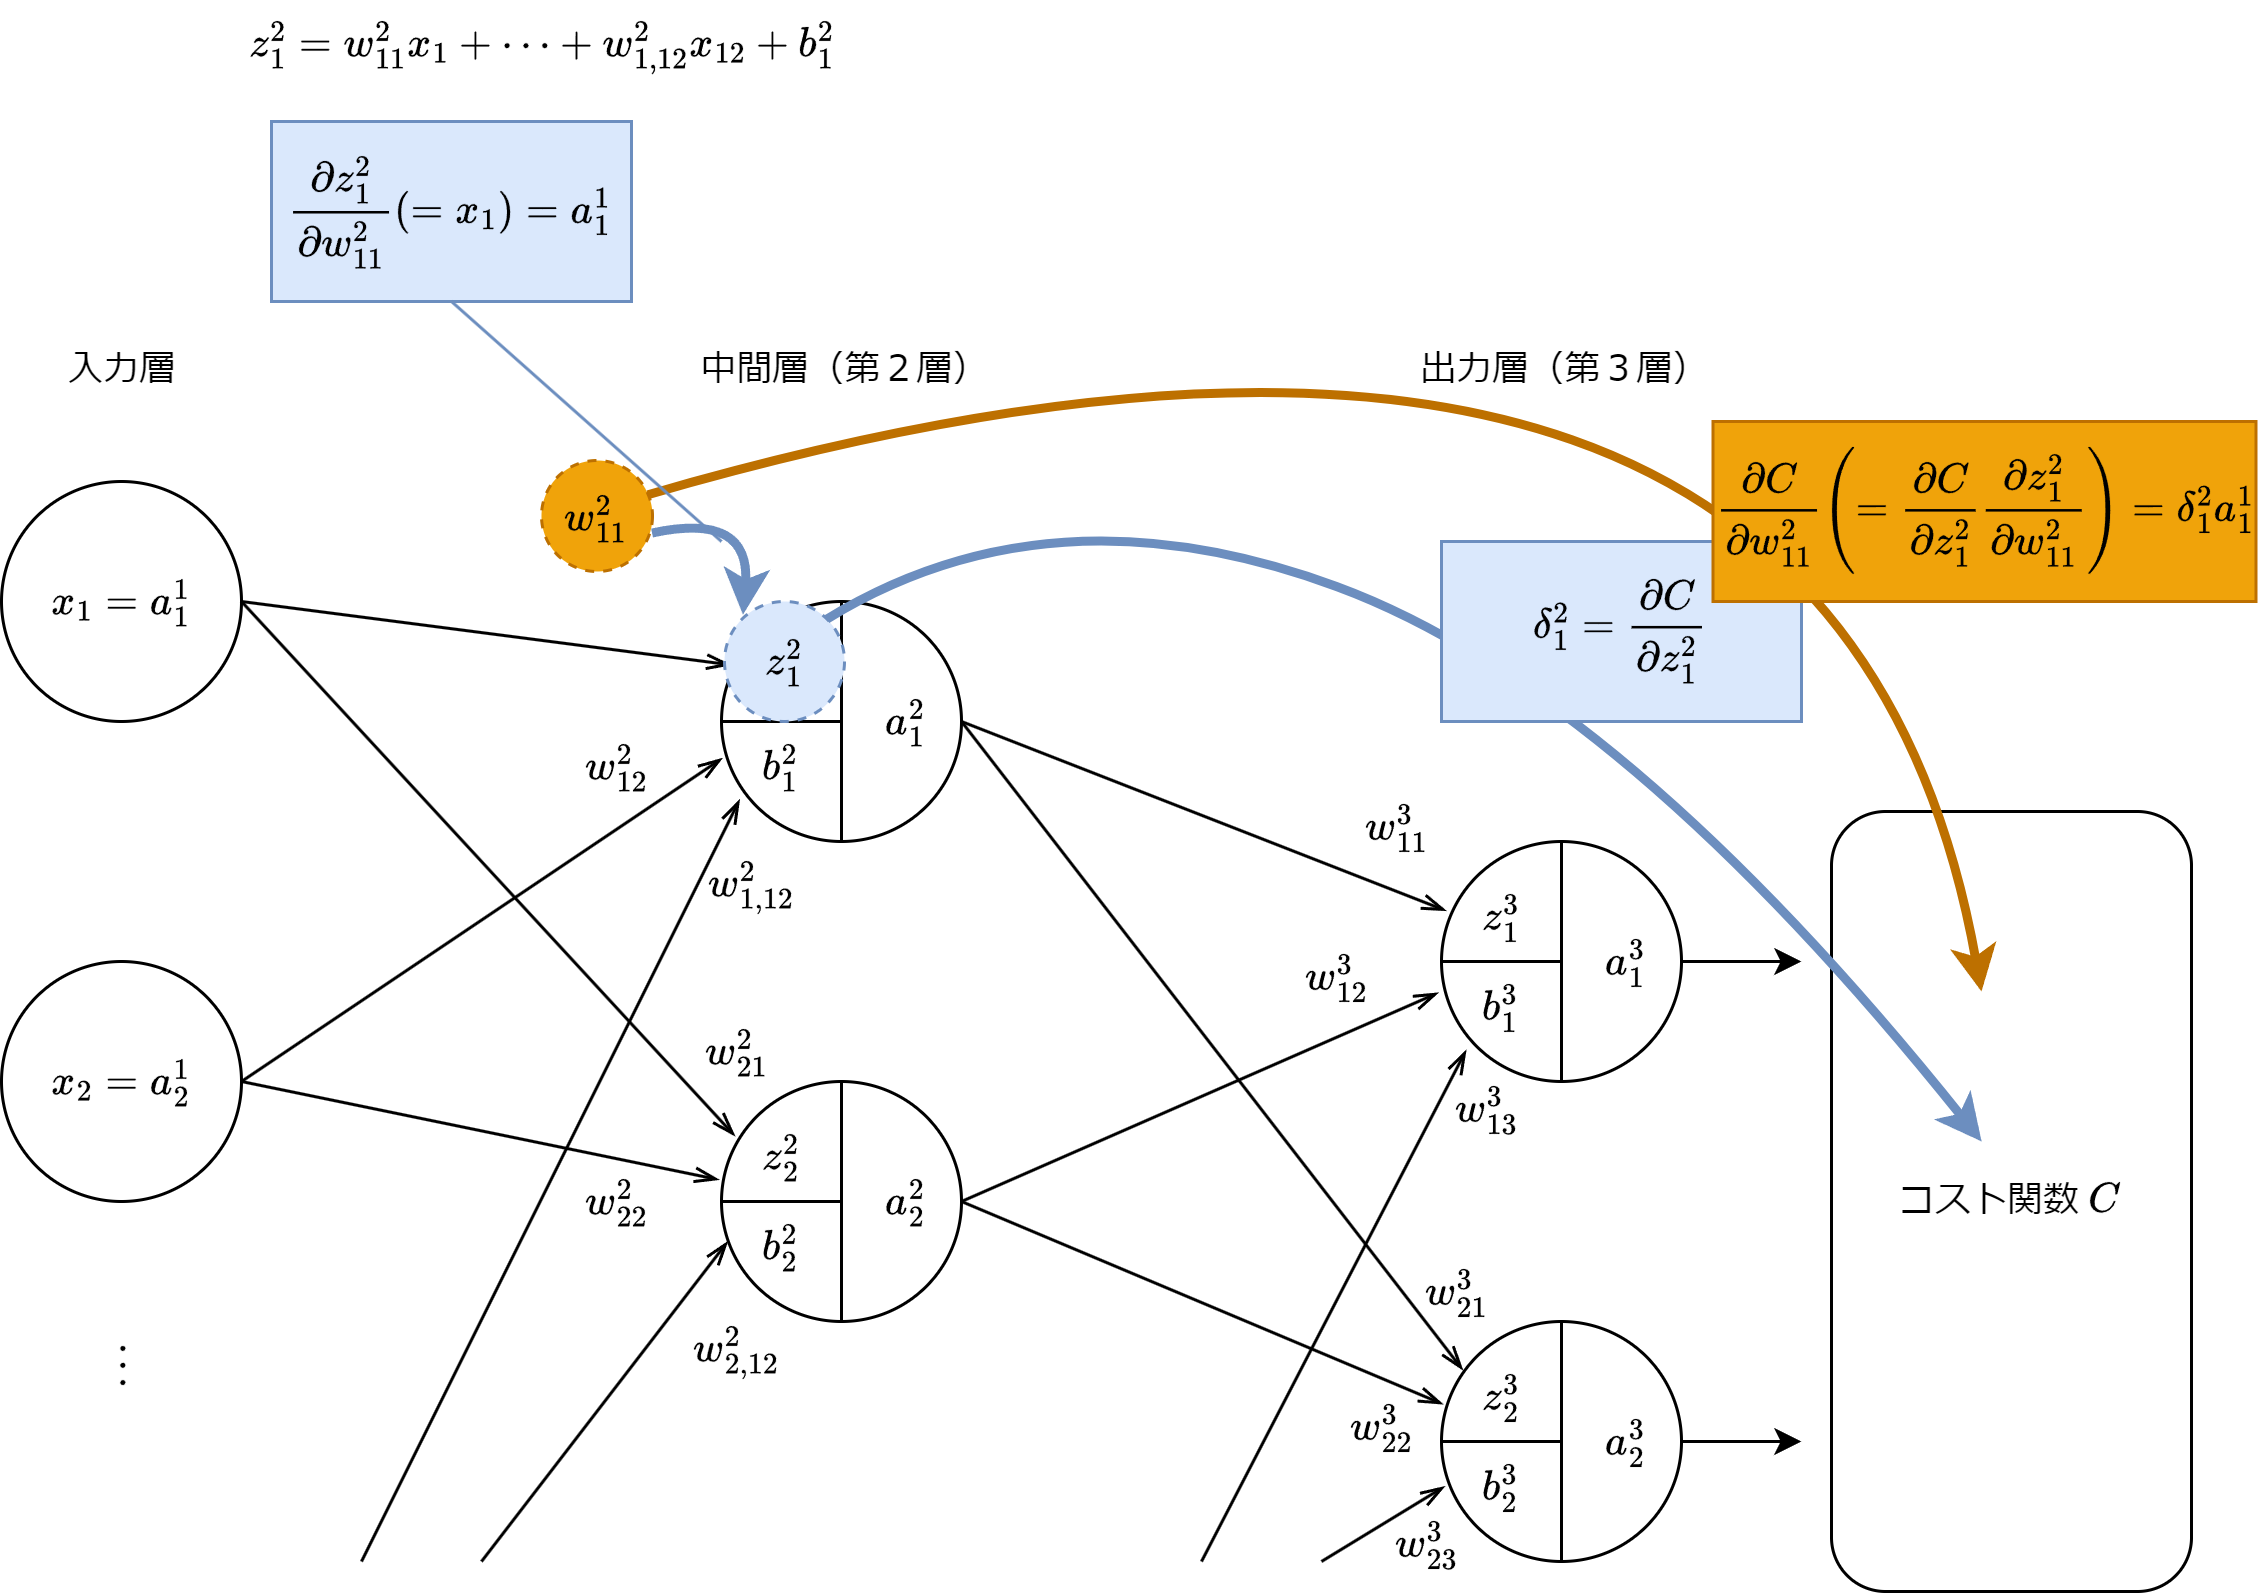
\includegraphics[width=0.7\linewidth]{img/image-of-the-partial-derivative-of-the-squared-error-with-respect-to-the-weights}
		\end{figure}
	\end{frame}
	\begin{frame}{バイアスに関する2乗誤差の偏微分を$ \delta^l_j $で表現}
		\begin{screen}
			バイアスに関する偏微分をユニットの誤差$ \delta^l_j $を用いて次にように表すことができる:
			\begin{equation}\label{eq:equation-expressing-the-partial-derivative-with-respect-to-the-bias-using-the-unit-error}
				\dfrac{\partial C}{\partial b^l_j} = \delta^l_j\quad (l \geq 2).
			\end{equation}
		\end{screen}
		ポイント
		\begin{itemize}
			\item $ \delta^l_j $の値さえ計算できれば、$ \dfrac{\partial C}{\partial b^l_j} $を偏微分の計算なしで求めることができる!
		\end{itemize}
	\end{frame}
	\begin{frame}{バイアスに関する2乗誤差の偏微分のイメージ}
		% TODO: \usepackage{graphicx} required
		\begin{figure}
			\centering
			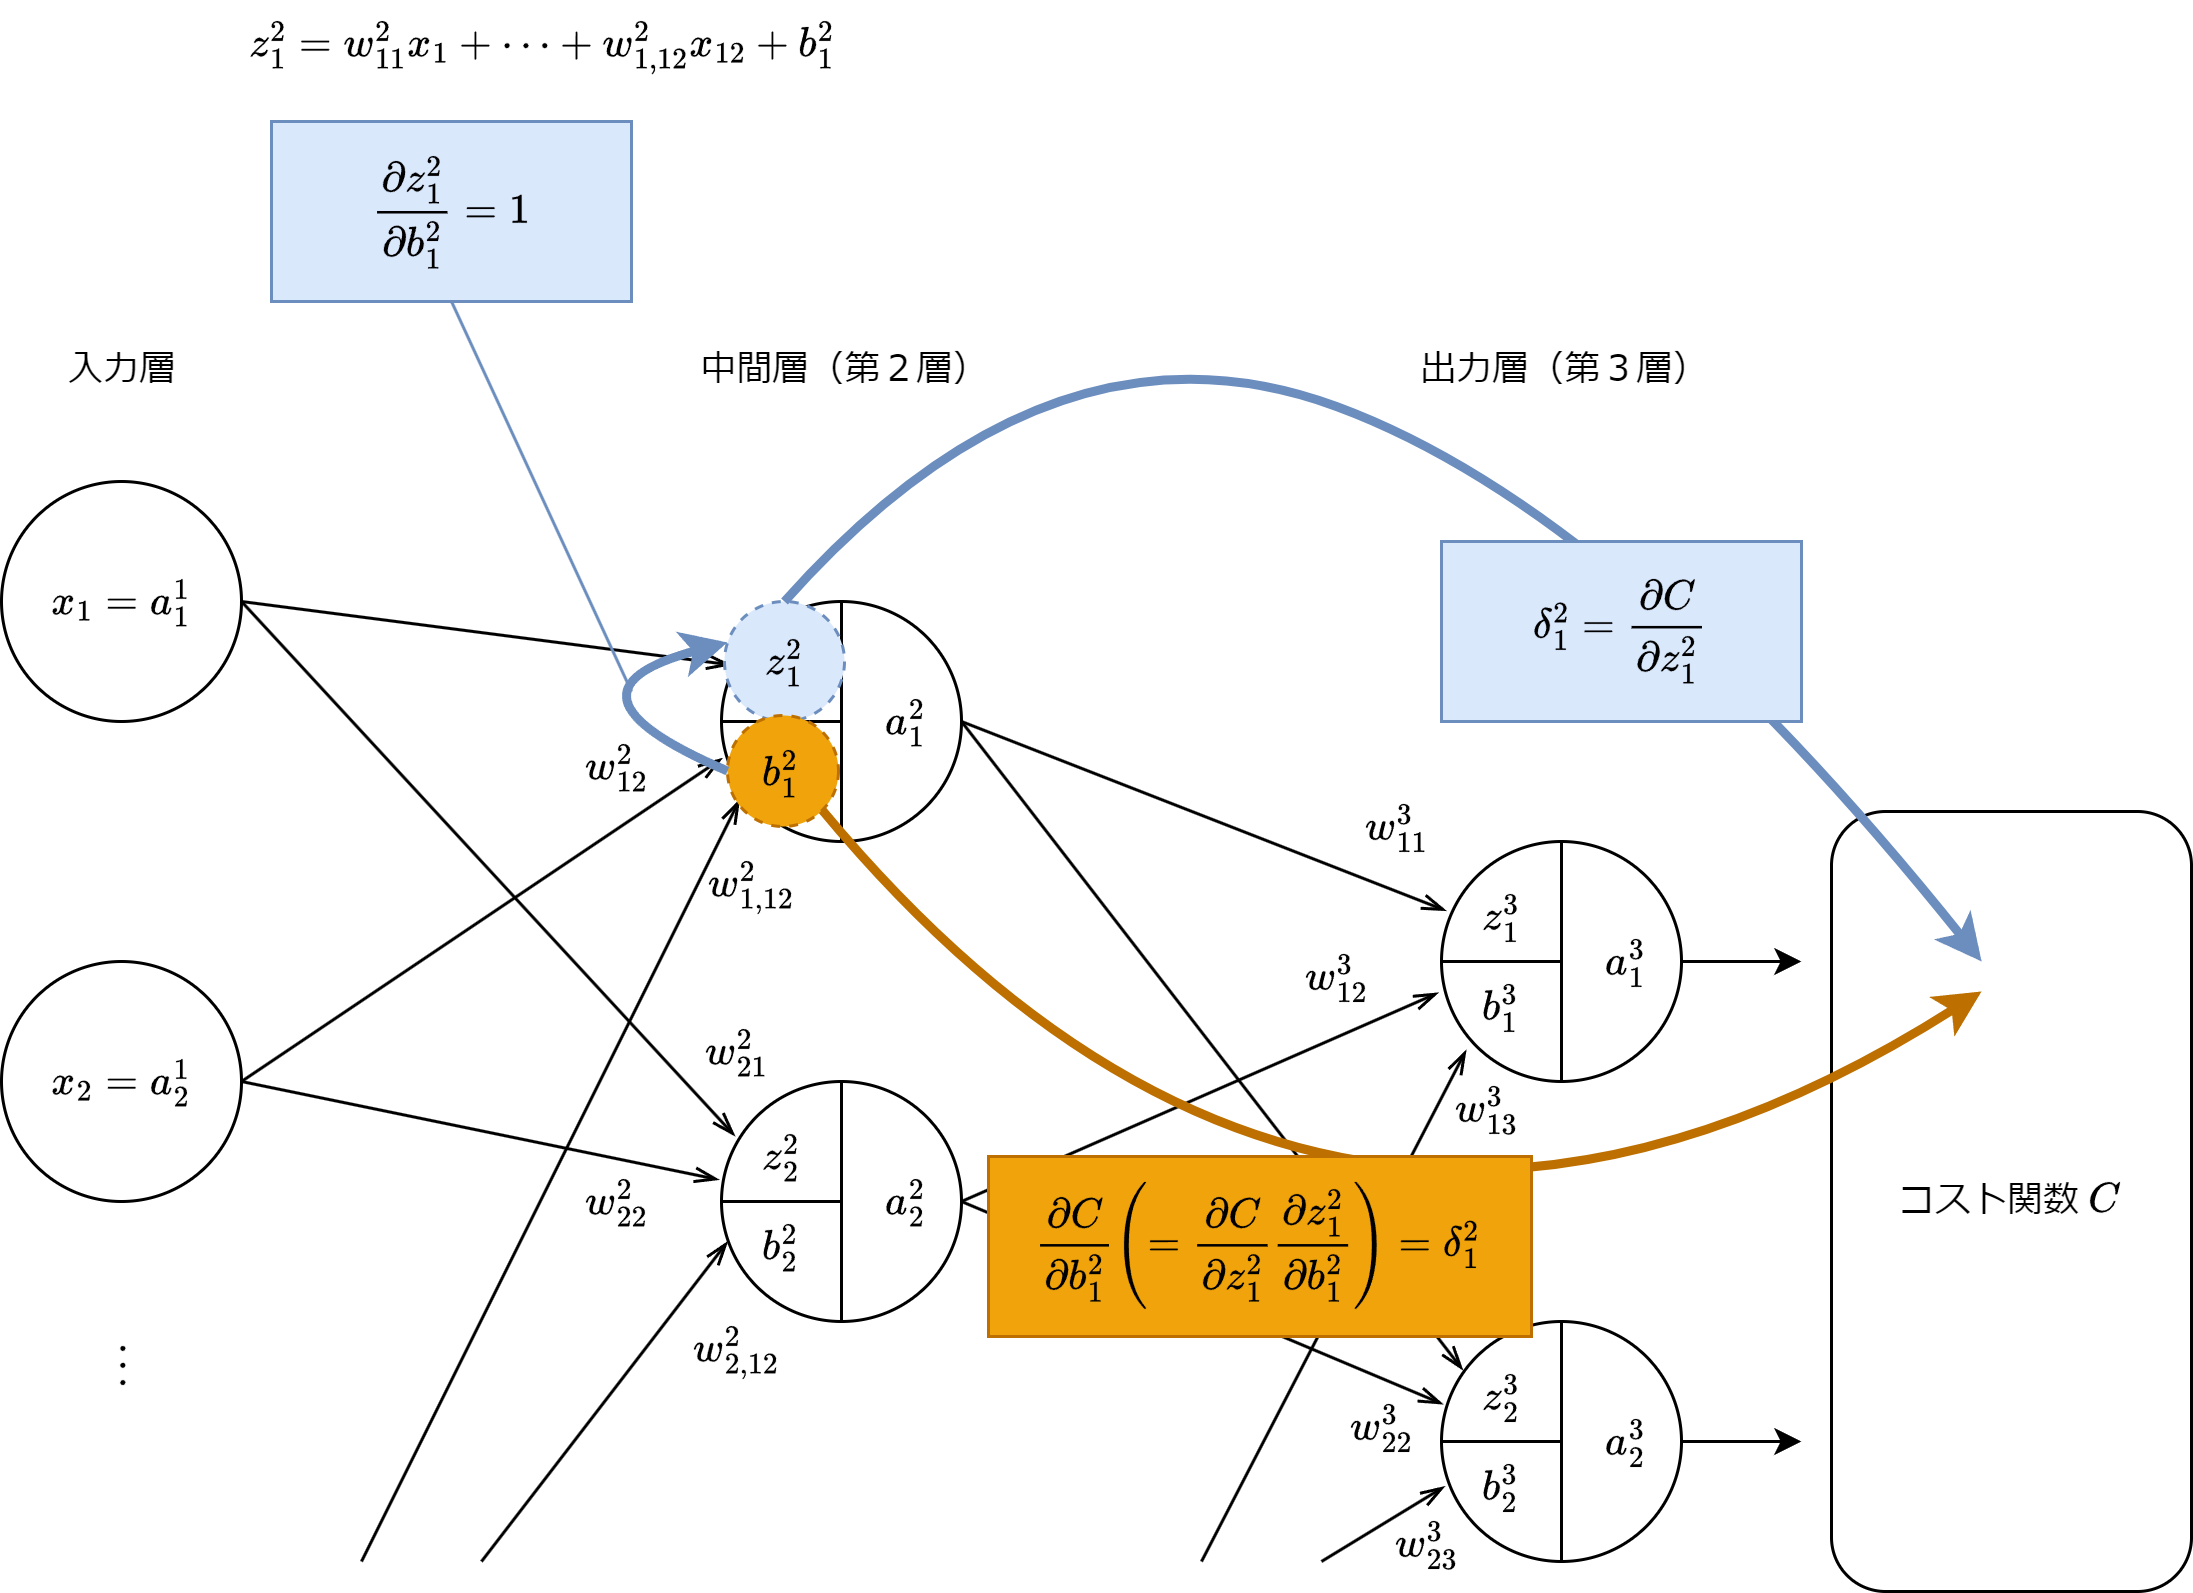
\includegraphics[width=0.7\linewidth]{img/image-of-the-partial-derivative-of-the-squared-error-with-respect-to-the-bias}
		\end{figure}
	\end{frame}
	\begin{frame}{で、$ \delta^l_j $はどう計算するの?}
		\underline{ここでようやく\alert{漸化式}の考え方が役立つ!}
		\begin{enumerate}
			\item 出力層(第$ L $層)のユニットの誤差$ \delta^L_j $を計算する
			\item $ l $層と$ l+1 $層のユニットの誤差の漸化式を用いて、出力層側のユニットの誤差から入力層側のユニットの誤差を計算する
		\end{enumerate}
		つまり、$ \delta^L_j $が計算できれば、$ \delta^{L-1}_j, \delta^{L-2}_j,\dots, \delta^2_j $とすべて計算できることになる
	\end{frame}
	\begin{frame}{出力層の$ \delta^L_j $を算出}
		
	\end{frame}
\end{document}
